\chapter{Tracker}

We considerate tracker as an algorithm used to detect a position of the object in
an image. We will present few tested trackers and their results in this task.
Firstly we provide a short description of simple straightforward tracker and
then we will describe more complicated trackers.

We use a word tracker generally for an algorithm able to detect object. Some
trackers but do not take an advantage of past images and information gained
from them. They simply detect an object in the each image. On the other hand
many good trackers using also information from previous images exist. For this
task some trackers from both categories.

%%%%%%%%%%%%%%%%%%%%%%%%%%%%%%%%%%%%%%%%%%%%%
\section {Detection based algorithms}

\subsection{Simple Background Tracker}

This tracker takes a photo of the background at the beginning and calls it
\emph{pattern}. In order to detect an object in \emph{image} is taken a
comparison of the \emph{image} and \emph{pattern}. A Comparison is done by
taking a sum of an absolute difference for each colour (Red, Green, Blue) in
the images. 

As result, we get a map, where higher values mean bigger difference between the
colors of the \emph{pattern} and \emph{image} at given point. We will assume it
is caused by an object in front of the camera at given point.  As the next step
we will binarize the map with a given \emph{treshold}. At this point we will
find a countour with biggest area using OpenCV library. Centerpoint of the
rectangle of this contour will be estimated position of our object in the
image..

\todo[inline]{Pomôže práve popísaný postup zapísať v niekoľkých riadkoch pseudokódu? Bolo
by to prehľadnejšie (na jedno pozretie jasné, bez čítania odstavca, ak čitateľ
vie, čo očakávať)}

\todo[inline]{Fotka vzoru (farebne), fotka s objektom, absolute\_diff, výsledok po rôznych tresholdoch}

\todo[inline]{Nájdenie contúr na obrázku, zobrazenie najväčšej, bod ako stred}

Advantages
\begin{itemize}
\item Quite straight-forward implementation
\item Ability to recognise variate object without having specific color or pattern.
\end{itemize}

Disadvantages
\begin{itemize}
\item Cannot recover from even small movement of the camera.
\item Moving object with a hand will cause recognizing the hand also as an object and will result wrongly estimated center of the moving object. Same problems cause shadows.
\end{itemize}

\subsection{Adaptive Background Tracker}

In order to make our background tracker robust to small movement of camera we
are going to update our \emph{pattern}. This could be simply done by defining \emph{pattern}
as the mean of last \emph{n} images.

Advantages
\begin{itemize}
\item Robust against movements of the camera
\end{itemize}

Disadvantages
\begin{itemize}
\item If the object is not moving it will disappear as becoming a part of the
background. After moving it will recover properly.
\end{itemize}

\subsection{HSV tracker}

This tracker is based on color tracking. Given an input object we find the
color with the largest area inside the object (range of color tones is used).
On position request we return a center of the largest area with given color
range.

We choose color coding via HSV (Hue, Saturation, Value). Unlike the RGB (Red,
Green, Blue) coding it can describe color as Hue value, not triple values of
mixed colors. The advantage of this approach is the fact that hue value is
preserved even though the color is lighter or darker (like shadows in the
image). On the other hand in RGB coding shadows may cause difference in all
three parts of coded color.

\begin{figure}\centering
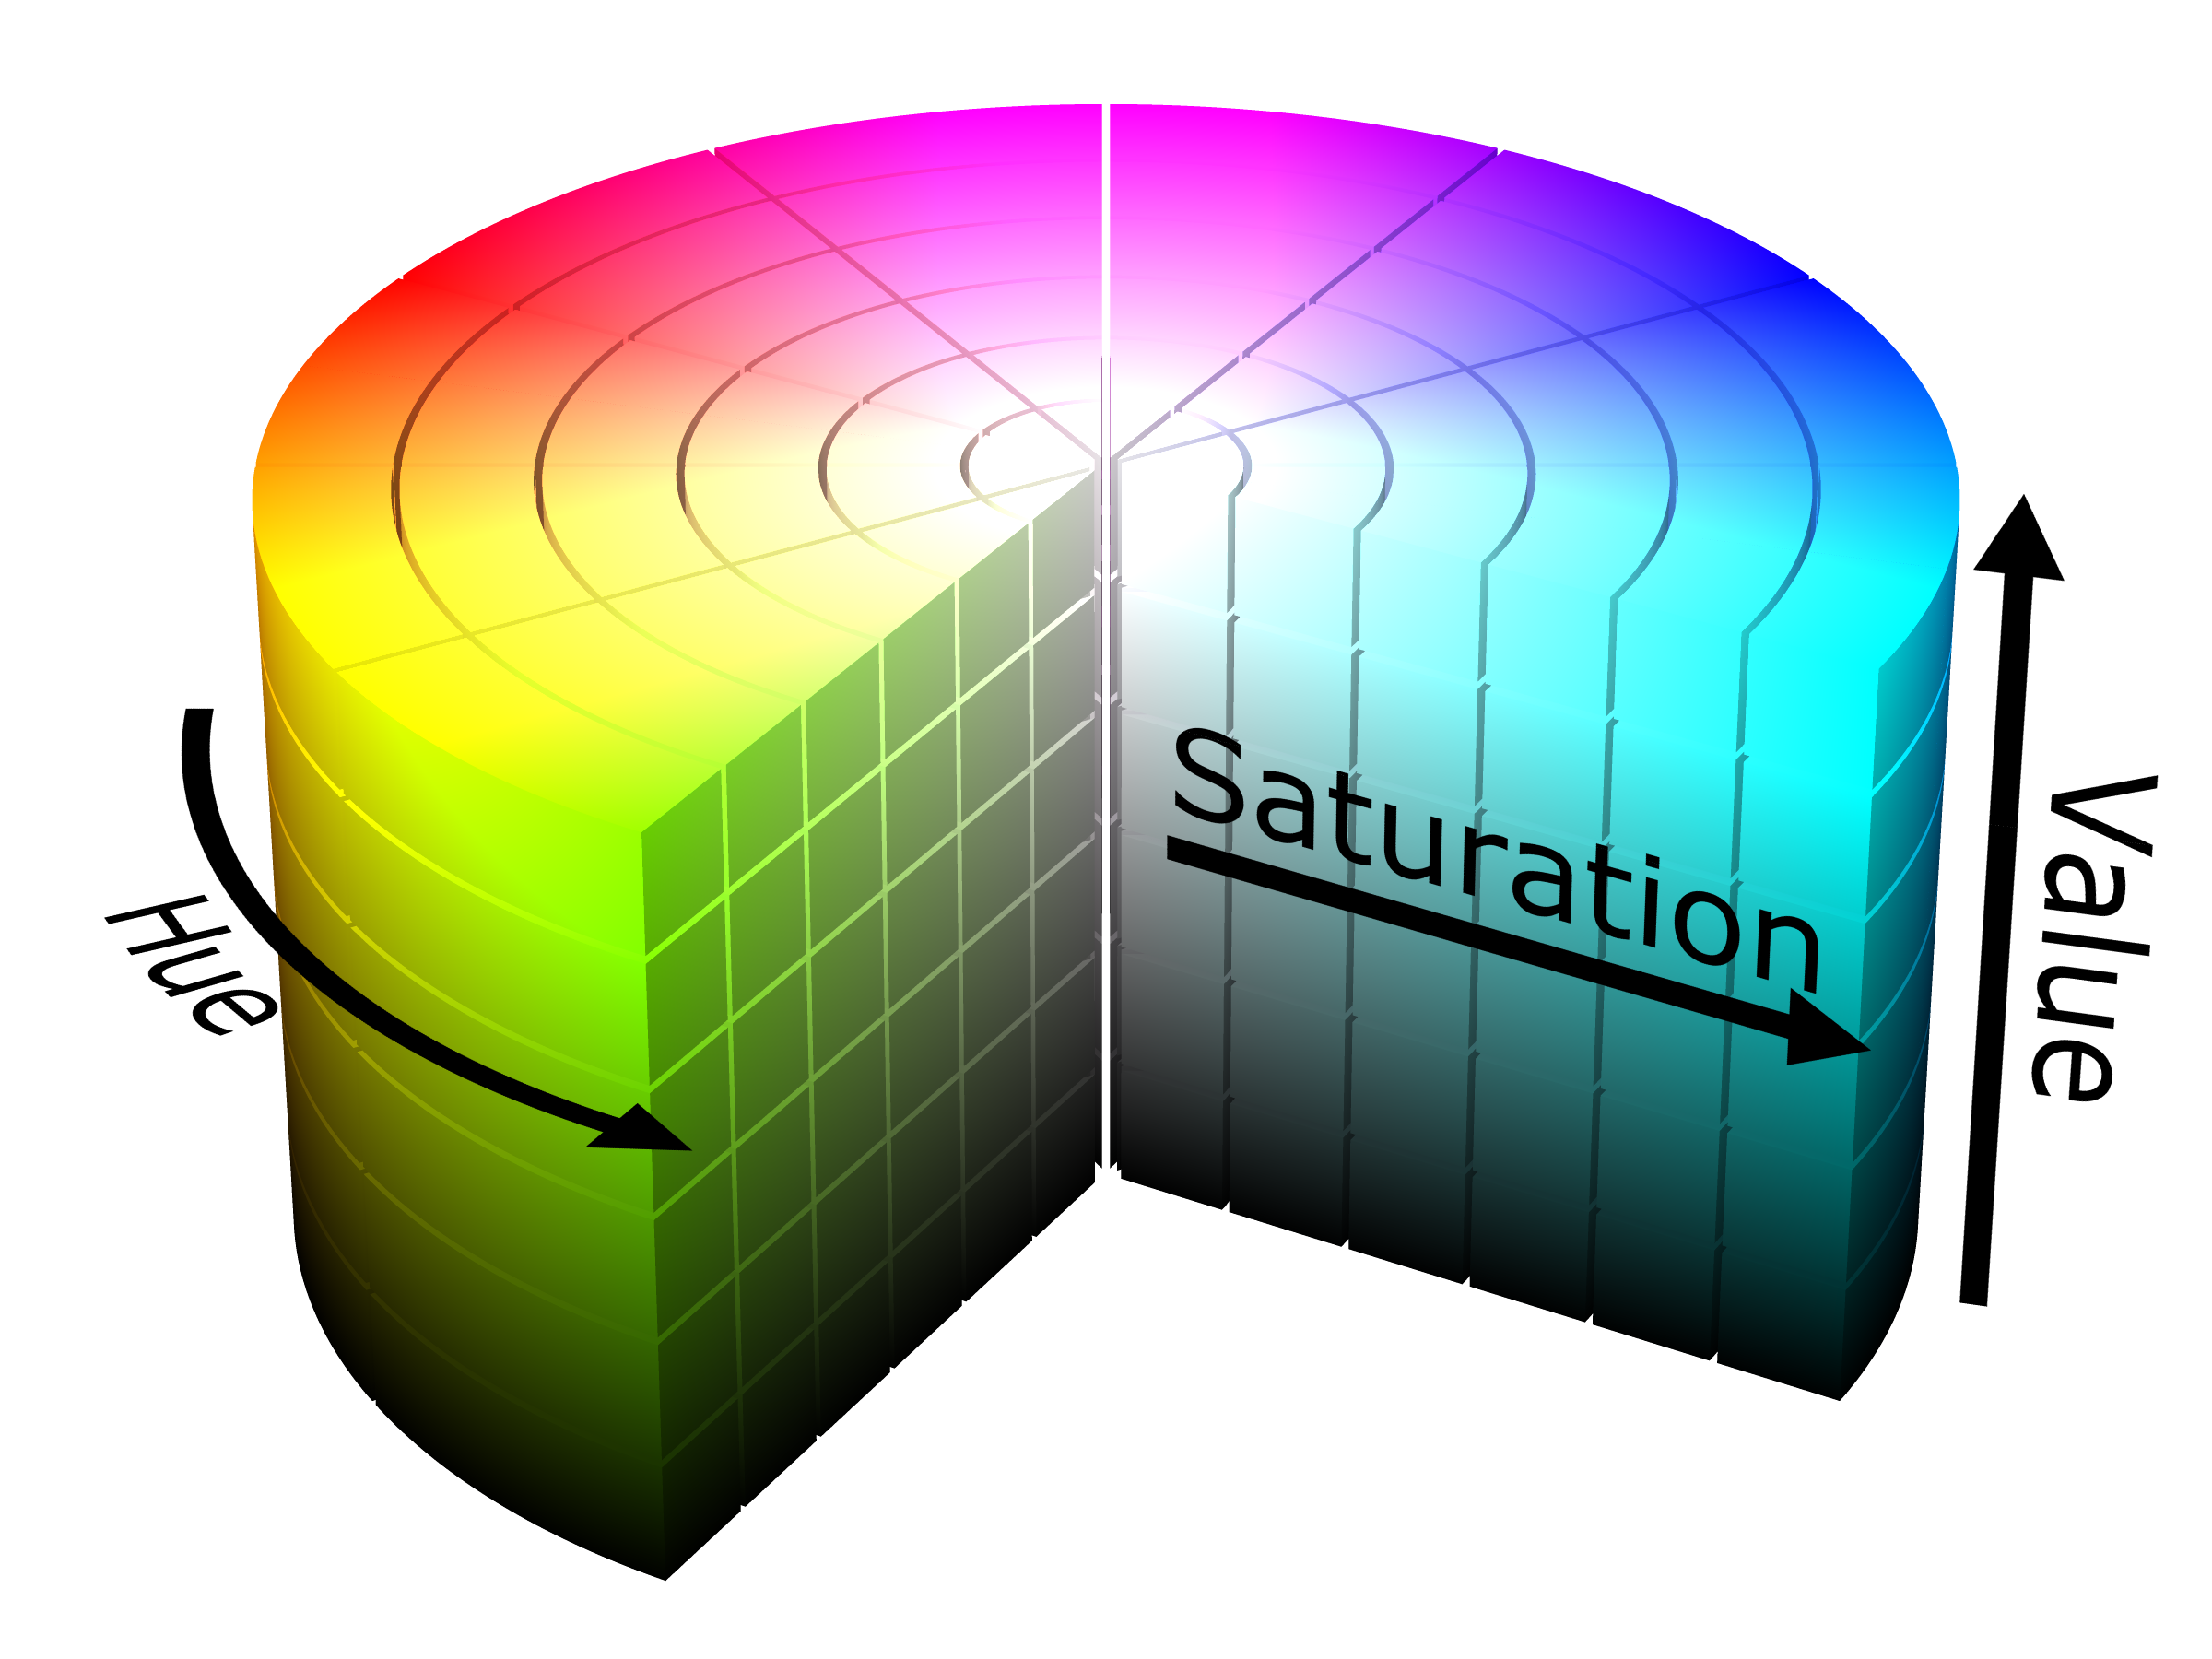
\includegraphics[width=0.65\textwidth]{img/hsv-cylinder.png}
\caption{"HSV cylinder" by SharkD is licensed under CC BY 3.0}
\end{figure}

Given image of template we convert from RGB to HSV. Then we choose an average color in the picture. Since the coding of Hue is placed on the circle, it is not enough to take common used average. It would cause that image full of Warm Red (Hue is circa equal to 15) and cool Red (Hue is circa 345) would average to mid cyan (Hue: 180).

In order to get more reasonable average we take hue value of each pixel as an angle. Then we use formulate to compute average of the angles.

$$ x = \sum cos \alpha $$
$$ y = \sum sin \alpha $$
$$ \alpha_{avg} = arctang2(y, x) $$

It is important to note, that results is only average, since geometric function have only really good approximation during computing.

\todo[inline]{Obrazok kde je maska a potom bod}

Disadvatages
- able to track only one color objects

\subsection {Pattern matching}

Pattern (or template) matching is based on sliding over the input image and comparing the template with the patch of the input image. TODO This algorithm is slow on big images. There for we preprocess the image beforehand by resizing it. At the other hand it may cause more false detection due to lower quality.

For patch and template comparison many different metrics may be used. We used TODO, since it perfomed best on given examples.

Metric could be written as:
$$R(x, y) = ....$$
where $x'$ and $y'$ denotes points from the neighbourhood of the $x, y$. $T$ denotes our pattern and $I$ denotes a patch from the input image. 

Advantages

Disadvantages
- not persistable against appearance changes -- really bad performance

%%%%%%%%%%%%%%%%%%%%%%%%%%%%%%%%%%%%%%%%%%%%%

\section{Tracking algorithms}

Using an advantage of information from previous frames could create not only
more stable but also faster trackers. Tracking preserves identity, which means
that also in the case multiple moving objects it remains tracking the original
one.

Sample information we can obtain from tracking information:
- velocity - from previous images we can estimate speed and the direction of
  the movement. This can reduce searching area to smaller one and increasing so
  the speed of the algorithm.
- appearance - object may rotate and change its shape or color. Tracker able to
  learn can be persistable against such changes

Algorithm using these information can cope with occlusion - what usually
detection algorithms are not able.

In the next sections we will present few trackers implemented in the OpenCV. We
provide short overview of the trackers available. At the end of the chapter
comparison table will be provided.

\subsection{BOOSTING tracker}
Boosting tracker is based on online AdaBoost. It consider bounding box as
positive sample and patches of background as negative ones. Given a new image,
classifier is run on every pixel in the neighbourhood of the previous location
and the score of the classifier is recorded. The location with highest score is
choosed as a new location. 

Advantages
- foundation of more successful trackers 

Disadvantages
- another trackers evolved from this idea and now perform better

H Grabner, M Grabner, and H Bischof, Real-time tracking via on-line boosting, In Proc. BMVC, volume 1, pages 47– 56, 2006
http://www.bmva.org/bmvc/2006/papers/033.pdf

\todo[inline]{Pridat do literatury https://www.learnopencv.com/object-tracking-using-opencv-cpp-python/}

\subsection{MIL tracker}
The shortcut comes from Multiple Instance Learning. In comparison to the
BOOSTING tracker, it does not keep only one image of positive example, but
whole bunch of the images. Small neighborhood of the current localition is took
as potential positive examples. It helps tracker to cope with the occlusion.

\subsection{KCF tracker}
KCF stands for Kernelized Correlation Filters. Similary as MIL tracker it uses
more positive samples and their larga overlapping regions. 

\subsection{TLD tracker}
Tracking, learning and detection, these are the three components of this
tracker. Tracker works frame to frame, detection corrects the tracker if
necessary. The learning estimates detector's errors and updates it to avoid
these errors in the future.

\subsection{MEDIANFLOW tracker}
Thi tracker focus on forward and backward measurements trying to minimize
discrepancies between these two trajectories.

\subsection{OpenCV note}
All these mentioned trackers are implemented in OpenCV contribute. GOTURN
tracker is also implemented in OpenCV, unfortunately at the time of the writing
thesis it contains bug causing it unusable.

%%%%%%%%%%%%%%%%%%%%%%%%%%%%%%%%%%%%%%%%%%%%%

\section{Comparison of trackers}

\subsubsection{Experiment with simplyfied environment}

Given a video sequence XYZ second long we studied an accuracy of trackers. The background is one colored and moving object is a red circle.

\todo[inline]{ Robot sledujúci čiaru do štvorca s červeným kruhom z vrchu (kamery sa dívajú zvrchu). Porovnanie bude uvedené ako čiary, ktoré sú nakreslené pomocou zachytených bodov.}

\subsubsection{Experiment in complex environment}

Background consistsed of many colors and patterns. Moving object has a pattern and is partially colored as the background.

\todo[inline]{ Vyskytli sa veci, ako, že stratil polohu? V akom percente? Mám ako rozumne vyjadriť presnosť tých súradníc lepšie než od oka?}
